\documentclass{article}
\newcommand{\template}{../../../template}
\usepackage{\template/packages}

\usepackage[english]{babel}

\newcommand{\titolo}{Analisi di \textit{Sentiment Penn TreeBank}}
\newcommand{\autore}{Rosso Carlo}
\newcommand{\data}{A.A. 2023/2024}
\newcommand{\corso}{Tesi}

\newcommand{\copertina}{
	\begin{titlepage}
		\begin{center}
			\vspace*{3cm}
			\LARGE{\textbf{\titolo}}\\
			\vspace{0.33cm}
			\Large{\textbf{\data}}\\
			\vspace{0.33cm}
			\Large{\autore}\\
		\end{center}
		\thispagestyle{empty}
	\end{titlepage}
}


% https://nlp.stanford.edu/sentiment/index.html

\begin{document}
\copertina

\tableofcontents
\newpage
\section{Introduction}

Sentiment classification is a form of text classification in which a piece of
text has to be classified into one of the predefined sentiment classes.
It is a supervised machine learning problem.
In fine-grained sentiment classification, there are five classes: very negative,
negative, neutral, positive, very positive (there is a nice pic to show this).\\
While transfer learning (pretraining and finetuning) has become the de-facto
standard in computer vision, NLP is yet to utilize this concept fully.\\
Recently Google reserchers published BERT (Bidirectional Encoder Representations
from Transformers), a deep bidirectional language model based on the Transformer
architecture.\\
In this paper, we use the pretrained BERT model and finetuen it for the
fine-grained sentiment classification task on the Stanford Sentiment Treebank
(SST-5) dataset.

\section{Summary from the paper}

Further progress towards understanding compositionality in tasks such as
sentiment detection requires riched supervised training and evaluation resources
and more powerful models of computation. Particularly, in this note, we will
discuss about the former. The authors introduce a Sentiment Treebank, which
includes fine grained sentiment labels for 215,154 phrases in the parse trees of
11,855 sentences. The \textit{Sentiment Penn Treebank} is the first corpus with
fully labeled parse trees tha allows for a complete analysis of the
compositional effects of sentiment in language.\\ 
The corpus is based on the dataset introduced by Pang and Lee (2005) and
consists of 11,855 sentences extracted from movie reviews. It was parsed with
the Stanford parser and includes a total of 215,154 unique phrases from those
parse trees, each annotated by 3 human judges.

\subsection{Origin}

It is considered the corpus of movie review excerpts from the
\texttt{rottentomatoes.com} website originally collected and published by Pang
and Lee (2005).
The original dataset includes 10.662 sentences, half of which were considered
positive and the other half negative.\\
The Stanford Parser (...) in used to parses all 10.662 sentences. In
approximately 1.100 cases it splits the snippet into multiple sentences. It was
used Amazon Mechanical Turk to label the resulting 215.154 phrases.\\
Starting at length 20, the majority are full sentences. One of the findings from
labeling sentences based on \textit{reader's perception} is that many of them
could be considered neutral.

\section{My analysis of the dataset}

According to ChatGPT at the start it is important to describe the dataset in
general, while most of the following information is already given in the
previous section, I will repeat those:
\begin{itemize}
	\item \textbf{Origin of the dataset}: \texttt{rottentomatoes.com}, then
		elaborated by Pang and Lee, the Stanford Parser, Amazon Mechanical Turk.
		Finally three judges were asked to decide on the final sentiment of the
		reviews. Note that the dataset is made of movie reviews;

	\item \textbf{Number of patterns}: 215.154 phrases from 10.662 sentences,
		but they are treated independently;

	\item \textbf{Number of classes}: 5: negative, somewhat negative, neutral,
		somewhat positive, positive. Actually the value given to each sentence
		ranges in 25 classes, but in the paper they are grouped in 5, since the
		most extreme values are not very common. I suppose I will use only 5;

	\item \textbf{Language}: English;
\end{itemize}

\subsection{Labels distribution}

\begin{figure}[H]
	\centering
	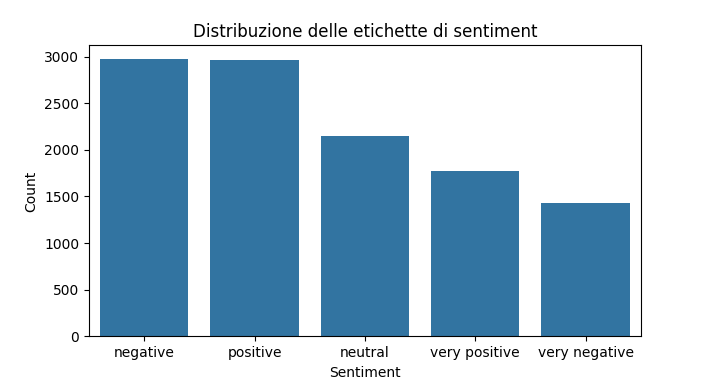
\includegraphics[width=0.8\textwidth]{figures/label_distribution.png}
	\caption{Labels distribution}
	\label{fig:labels_distribution}
\end{figure}

Back to the actual numbers, we got the following distribution:
\begin{itemize}
	\item \textbf{Negative}: 1432;
	\item \textbf{Somewhat negative}: 2971;
	\item \textbf{Neutral}: 2144;
	\item \textbf{Somewhat positive}: 2966;
	\item \textbf{Positive}: 1773;
\end{itemize}

\subsection{Texts length distribution}

\begin{figure}[H]
	\centering
	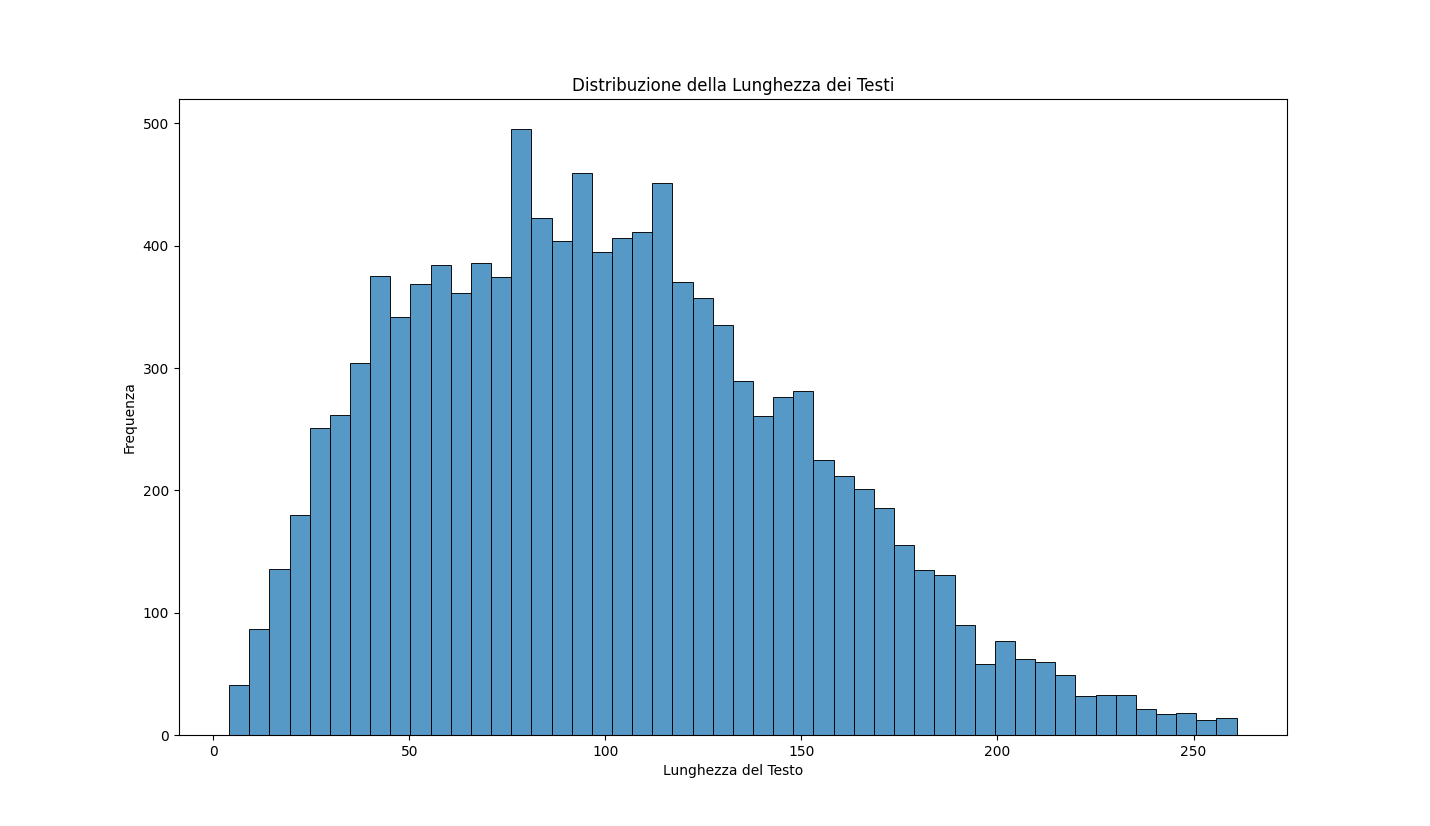
\includegraphics[width=0.8\textwidth]{figures/text_length.png}
	\caption{Texts length distribution}
	\label{fig:text_length_distribution}
\end{figure}

Where the mean of the texts length is 101 and the median is 97.

\subsection{Most frequent words}

\begin{figure}[H]
	\centering
	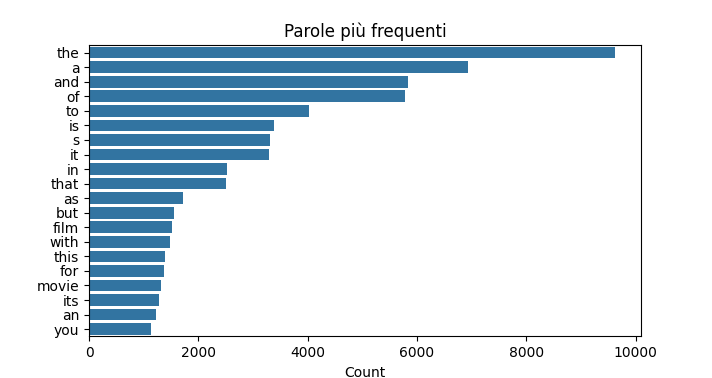
\includegraphics[width=0.8\textwidth]{figures/most_frequent_words.png}
	\caption{Most frequent words}
	\label{fig:most_frequent_words}
\end{figure}

Finally the most frequent words are:
\begin{itemize}
	\item \textbf{the}: 9615;
	\item \textbf{a}: 6934;
	\item \textbf{and}: 5841;
	\item \textbf{of}: 5787;
	\item \textbf{to}: 4033;
\end{itemize}

\subsection{Sentiment visualization}

The sentiment visualization is done through word clouds, where the size of the
word is proportional to the frequency of the word in the dataset, within the
label. The following figures show the word clouds for each label.

\begin{figure}[H]
	\centering
	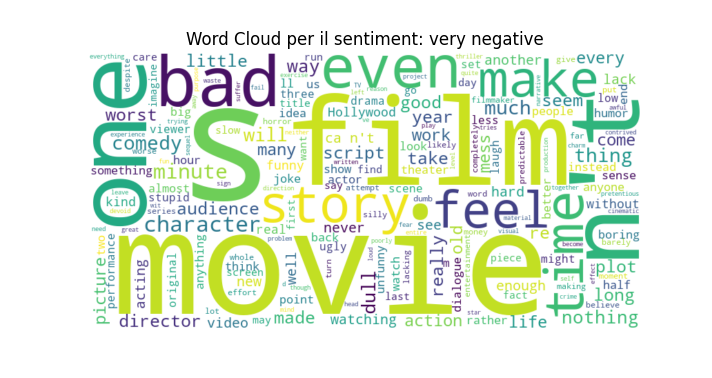
\includegraphics[width=0.8\textwidth]{figures/wordcloud_negative.png}
	\caption{Negative word cloud}
	\label{fig:negative_word_cloud}
\end{figure}

\begin{figure}[H]
	\centering
	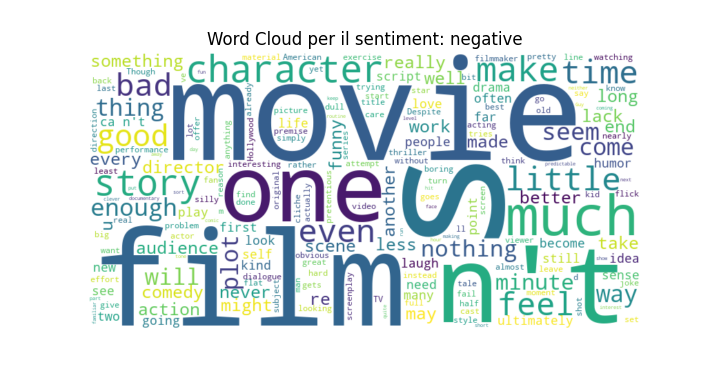
\includegraphics[width=0.8\textwidth]{figures/wordcloud_snegative.png}
	\caption{Somewhat negative word cloud}
	\label{fig:somewhat_negative_word_cloud}
\end{figure}

\begin{figure}[H]
	\centering
	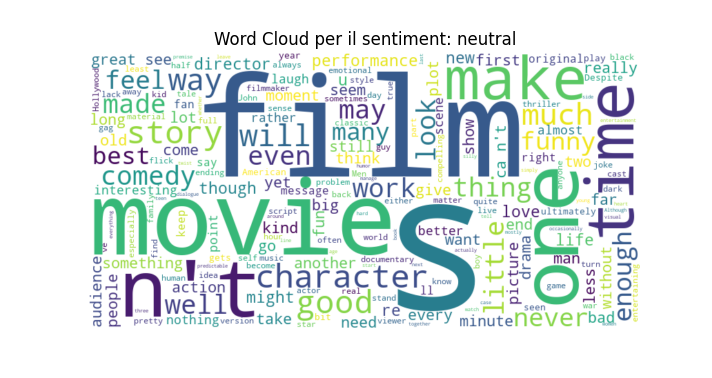
\includegraphics[width=0.8\textwidth]{figures/wordcloud_neutral.png}
	\caption{Neutral word cloud}
	\label{fig:neutral_word_cloud}
\end{figure}

\begin{figure}[H]
	\centering
	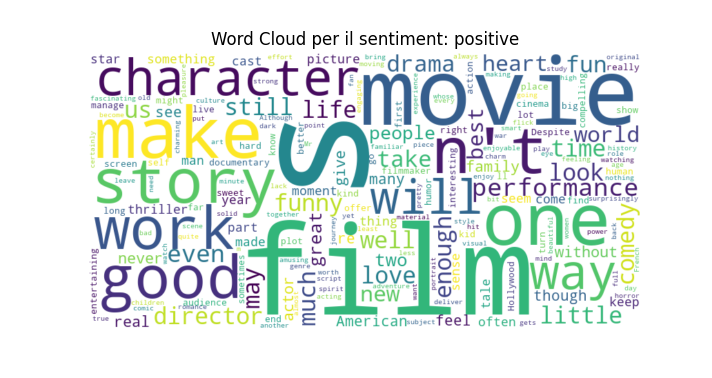
\includegraphics[width=0.8\textwidth]{figures/wordcloud_spositive.png}
	\caption{Somewhat positive word cloud}
	\label{fig:somewhat_positive_word_cloud}
\end{figure}

\begin{figure}[H]
	\centering
	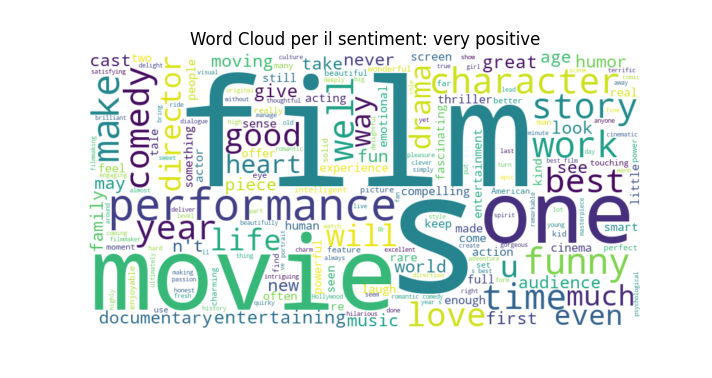
\includegraphics[width=0.8\textwidth]{figures/wordcloud_positive.png}
	\caption{Positive word cloud}
	\label{fig:positive_word_cloud}
\end{figure}

\section{Integrations}

\begin{itemize}
	\item \textbf{Vocabulary dimension}
\end{itemize}


\end{document}
